\documentclass{article}

\usepackage{indentfirst}
\usepackage{setspace}
\doublespacing

% Packages for showing source code
\usepackage{listings}
\usepackage{color}

\definecolor{dkgreen}{rgb}{0,0.6,0}
\definecolor{gray}{rgb}{0.5,0.5,0.5}
\definecolor{mauve}{rgb}{0.58,0,0.82}

\lstset{frame=tb,
language=C,
aboveskip=1mm,
belowskip=1mm,
showstringspaces=false,
columns=flexible,
basicstyle={\small\ttfamily},
numbers=none,
numberstyle=\tiny\color{gray},
keywordstyle=\color{blue},
commentstyle=\color{dkgreen},
stringstyle=\color{mauve},
breaklines=true,
breakatwhitespace=true,
tabsize=3
}

% Package for flowcharts/diagrams

\usepackage{tikz}
\usetikzlibrary{shapes.geometric, arrows}

\tikzstyle{startstop} = [rectangle, rounded corners, minimum width=3cm, minimum height=1cm,text centered, draw=black, fill=red!30]
\tikzstyle{io} = [rectangle, minimum width=3cm, minimum height=1cm,text centered, draw=black, fill=blue!30]
\tikzstyle{process} = [diamond, minimum width=2cm, minimum height=0cm, text centered, draw=black, fill=orange!30]
\tikzstyle{arrow} = [thick,->,>=stealth]

% ==================================================
% Begin Paper
% ==================================================

\title{Fully Generalized Compilation}
\date{01-26-2017}
\author{Lucas Saldyt}

\begin{document}

\maketitle
\pagenumbering{gobble}
\newpage
\pagenumbering{arabic}

\section{Abstract}

Assuming that two languages are \textit{isomorphic}, one syntax can be converted to another if given an adequate description of each syntax's grammar.
At an abstract level, this conversion is entirely practical. 
Progtran is an investigation into the feasibility of a \textbf{Fully Generalized Compiler}, a multi-language source-to-source compiler. 
Given source code in one language, a description of its grammar \textbf{A} , and a description of an output language's grammar \textbf{B}, can \textbf{A} be converted to \textbf{B} such that the output in \textbf{B} is indistinguishable from a program originally written in \textbf{B}?

\section{Introduction}

A \textbf{Full Generalized Compiler} is a tool for programming language researchers, providing a \textit{dynamic framework} for easily modifying syntax of input and output languages. 
A new programming language can even be fully implemented without recompiling the software. 
Progtran also uses this concept (user defined dynamic grammars) to re-implement existing source-to-source compilation tools, such as \textbf{Cython} or \textbf{2to3}.

\section{Methods}


\subsection{Grammars}
\subsection{Constructors}
\subsection{AST Transformations}

\newpage

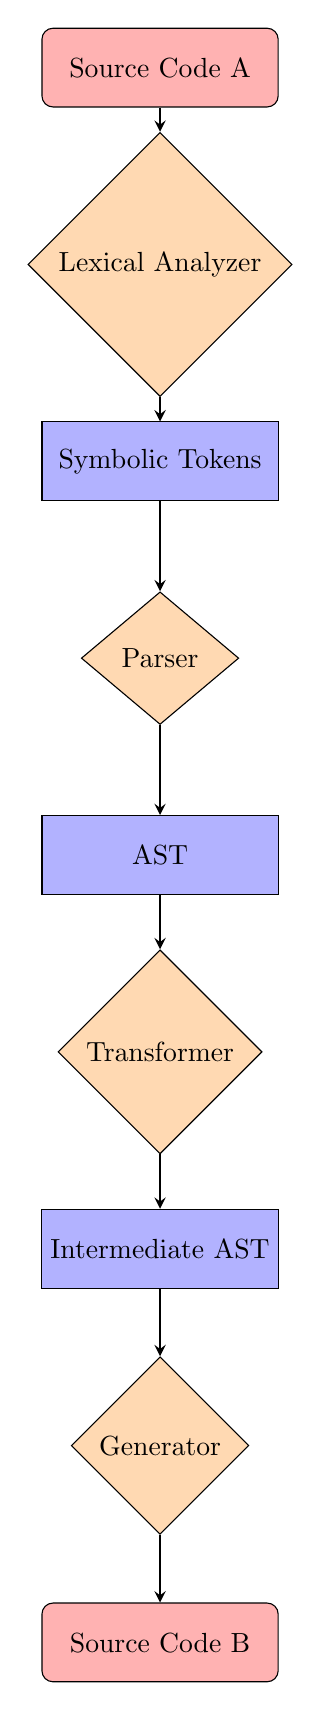
\begin{tikzpicture}[node distance=2.5cm]

    \node (sourcea) [startstop]                 {Source Code A};
    \node (lexer)   [process, below of=sourcea] {Lexical Analyzer};
    \node (tokens)  [io, below of=lexer]        {Symbolic Tokens};
    \node (parser)  [process, below of=tokens]  {Parser};
    \node (asta)    [io, below of=parser]       {AST};
    \node (trans)   [process, below of=asta]    {Transformer};
    \node (astb)    [io, below of=trans]        {Intermediate AST};
    \node (gen)     [process, below of=astb]    {Generator};
    \node (stop)    [startstop, below of=gen]   {Source Code B};


    \draw [arrow] (sourcea) -- (lexer);
    \draw [arrow] (lexer) -- (tokens);
    \draw [arrow] (tokens) -- (parser);
    \draw [arrow] (parser) -- (asta);
    \draw [arrow] (asta) -- (trans);
    \draw [arrow] (trans) -- (astb);
    \draw [arrow] (astb) -- (gen);
    \draw [arrow] (gen) -- (stop);

\end{tikzpicture}


\section{Results}
\subsection{Quicksort Cython Comparison}

This is not meant to be a robust benchmark. Instead, it aims to show that Cython and Transpilation yield similar results.

Output for 1000 sorting iterations:
\begin{center}
    \begin{verbatim}
        Transpile speedup:
        13.335545461765733
        Cython speedup:
        13.9866371311344
        Transpile : Cython comparison (1> indicates transpile is faster than cython)
        0.9534490197132998
    \end{verbatim}
\end{center}

\newpage
\subsection{Original Python Code}

\lstset{language=Python}
\begin{lstlisting}
def sort(array):
    less    = []
    equal   = []
    greater = []

    if len(array) <= 1:
        return array
    else:
        pivot = array[0]
        for x in array:
            if x < pivot:
                less.append(x)
            if x == pivot:
                equal.append(x)
            if x > pivot:
                greater.append(x)
        return sort(less) + equal + sort(greater)

def main():
    l = sort([3, 2, 12, 9, 4, 68, 17, 1, 2, 3, 4, 5, 6, 12, 9  , 8, 7, 6,5, 4, 743])

if __name__ == "__main__":
    main()
\end{lstlisting}

\lstset{language=C}

\newpage
\subsection{Generated C++ Code (Glossa)}

\begin{lstlisting}
#include "../std/std.hpp"
template <typename T_array>
auto sort (T_array array)
{
    auto less = std::vector<Object>({});
    auto equal = std::vector<Object>({});
    auto greater = std::vector<Object>({});
    if (len(array) <= 1)
    {
        return array;
    }
    else
    {
        auto pivot = array[0];
        for (auto x : array)
        {
            if (x < pivot)
            {
                less.push_back(x);
            }
            if (x == pivot)
            {
                equal.push_back(x);
            }
            if (x > pivot)
            {
                greater.push_back(x);
            }
        };
        return sort(less) + equal + sort(greater);
    };
}
\end{lstlisting}

\newpage
\subsection{Generated C Code (Cython)}

Generated code for Cython is much more complex, as it integrates with the Python FFI

For example, this snippet declares an empty array

\begin{lstlisting}
  /* "main.py":6
 *     Sorts an array of comparable values
 *     """
 *     less    = []             # <<<<<<<<<<<<<<
 *     equal   = []
 *     greater = []
 */
  __pyx_t_1 = PyList_New(0); if (unlikely(!__pyx_t_1)) {__pyx_filename = __pyx_f[0]; __pyx_lineno = 6; __pyx_clineno = __LINE__; goto __pyx_L1_error;}
  __Pyx_GOTREF(__pyx_t_1);
  __pyx_v_less = ((PyObject*)__pyx_t_1);
  __pyx_t_1 = 0;
\end{lstlisting}

\end{document}
